\documentclass[utf8]{frontiersSCNS}
\usepackage{url,hyperref,lineno,microtype,subcaption}
\usepackage{color,tensor,multirow,siunitx}
\usepackage[onehalfspacing]{setspace}
\usepackage{makecell}

\renewcommand{\cellalign}{cl}

\newcommand{\ds}{\displaystyle}
\newcommand{\nl}{\ \\ }
\newcommand{\ud}{\textrm{ d}}
\newcommand{\bs}{\bigskip}

\newcommand{\bu}{\mathbf{u}}
\newcommand{\bv}{\mathbf{v}}
\newcommand{\bx}{\mathbf{x}}
\newcommand{\be}{\mathbf{e}}
\newcommand{\bb}{\mathbf{b}}
\newcommand{\bk}{\mathbf{k}}
\newcommand{\bn}{\mathbf{n}}
\newcommand{\bR}{\mathbf{R}}

\definecolor{red}{rgb}{1,0,0}
\definecolor{blue}{rgb}{0,0,0.8}
\definecolor{green}{rgb}{0,0.5,0}
\newcommand{\emphc}[1]{\emph{\textcolor{red}{#1}}}
\newcommand{\replyRone}[1]{\emph{\textcolor{blue}{#1}}}
\newcommand{\replyRtwo}[1]{\emph{\textcolor{green}{#1}}}
\newcommand{\modif}[1]{\textcolor{red}{#1}}
\newcommand{\hycom}{\textsc{hycom} }
\newcommand{\slim}{\textsc{slim}\ }
\newcommand{\ie}{{\it i.e.}\ }
\newcommand{\eg}{{\it e.g.}\ }
\linenumbers

\def\keyFont{\fontsize{8}{11}\helveticabold }
\def\firstAuthorLast{Dobbelaere {et~al.}} %use et al only if is more than 1 author
\def\Authors{Thomas Dobbelaere\,$^{1,*}$, Erinn Muller\,$^{2}$, Lewis Gramer\,$^{3,4}$, Dan Holstein\,$^{5}$  and Emmanuel Hanert\,$^{1,6}$}
\def\Address{
$^{1}$ Earth and Life Institute (ELI), UCLouvain, Louvain-la-Neuve, Belgium \\
$^{2}$ Coral Health and Disease Program, Mote Marine Laboratory, Sarasota, FL, USA \\
$^{3}$ Cooperative Institute for Marine and Atmospheric Studies (CIMAS), University of Miami, Miami, FL, USA \\
$^{4}$ Atlantic Oceanographic and Meteorological Laboratory (AOML), NOAA, Miami, FL, USA \\
$^{5}$ Department of Oceanography and Coastal Sciences, College of the Coast and Environment, Louisiana State University, Baton Rouge, LA, USA \\
$^{6}$ Institute of Mechanics, Materials and Civil Engineering (IMMC), UCLouvain, Louvain-la-Neuve, Belgium \\
}
% The Corresponding Author should be marked with an asterisk
% Provide the exact contact address (this time including street name and city zip code) and email of the corresponding author
\def\corrAuthor{Earth and Life Institute (ELI), UCLouvain, Croix du Sud 2 box L7.05.16, B-1348 Louvain-la-Neuve, Belgium}

\def\corrEmail{thomas.dobbelaere@uclouvain.be}


\begin{document}
\onecolumn
\firstpage{1}

\title[Propagation of SCTLD in Florida]{Modeling the propagation of the Stony-Coral-Tissue-Loss disease in Florida}

\author[\firstAuthorLast ]{\Authors} %This field will be automatically populated
\address{} %This field will be automatically populated
\correspondance{} %This field will be automatically populated
\extraAuth{}

\maketitle
\begin{abstract}

For about six years, the Florida Reef Tract (FRT) has been experiencing an outbreak of the Stony Coral Tissue Loss Disease (SCTLD). First reported off the coast of Miami-Dade County in 2014, the SCTLD outbreak now \emphc{(In April 2020?)} spans from the northern extent of the reef tract in Martin County down to Rock Key in the Lower Keys. However, the causative agent for this outbreak is currently unknown. Here we show how a high-resolution bio-physical model can inform on the potential characteristics of the causative agent of the disease and its vector. In this study, the agent is assumed to be transported within composite material (such as coral mucus, dying tissues and/or resuspended sediments) driven by currents and potentially persisting in the water column for extended periods of time. In this framework, our simulations suggest that the SCTLD is likely to be propagated within neutrally buoyant materials driven by mean barotropic currents. Calibration of our model parameters with field data show that corals are then infected within a mean transmission time of 6.45. Furthermore, the propagation speed of the disease through the FRT is shown to be very sensitive to the proportion of infected corals that colonies can sustain before the development of an outbreak. Our results present a new connectivity-based approach to understand the spread of the SCTLD through the FRT. Such method can provide a valuable complement to field observations and lab experiments to support the management of the epidemic as well as the identification of its causative agent. 

\tiny
\keyFont{ \section{Keywords:} stony-coral-tissue-loss disease, biophysical modeling, Florida reef tract, spatial epidemiology, connectivity} 
\end{abstract}

% === INTRODUCTION === %
\section{Introduction}
Stony Coral Tissue Loss disease: where, when, what do we know (tank based transmission exp, spatial modeling paper)
SIR modeling background?
Hydrodynamic modeling?
The objective...

% === METHODS === %
\section{Methods}

% --> Subsection 1
\subsection{Modeling reef connectivity}
The exchanges of infectious material between coral reefs are primarily driven by ocean currents, which therefore have to be accurately simulated. An ocean model should provide a realistic large-scale circulation while also resolving small-scale flow features down to the scale of individual reefs. In this study, we use the unstructured-mesh depth-integrated coastal ocean model SLIM\footnote{{\tt https://www.slim-ocean.be}} to simulate ocean currents over an area that includes the FRT but also the Florida Strait and part of the Gulf of Mexico (Fig. \ref{fig:setup}). By using an unstructured mesh, we can increase the model resolution only over the FRT and hence concentrate computational resources where they are most needed. SLIM, being a depth-averaged model, is well suited to shallow-water flows. %On the shelf break and in deeper areas, it might however not be able to model more complex processes such as mesoscale eddies that are observed along the southern flank of the FRT and the thermally-driven FC. This issue has been partly circumvented by relaxing SLIM's velocity towards the depth-averaged velocity obtained with the HYbrid Coordinate Ocean Model (HYCOM, \cite{Chassignet2007}) implemented over the Gulf of Mexico, when the water depth exceeds a certain threshold.
Details of the model formulation and validation are provided in \cite{frys20}. 

\begin{figure}
    \centering
    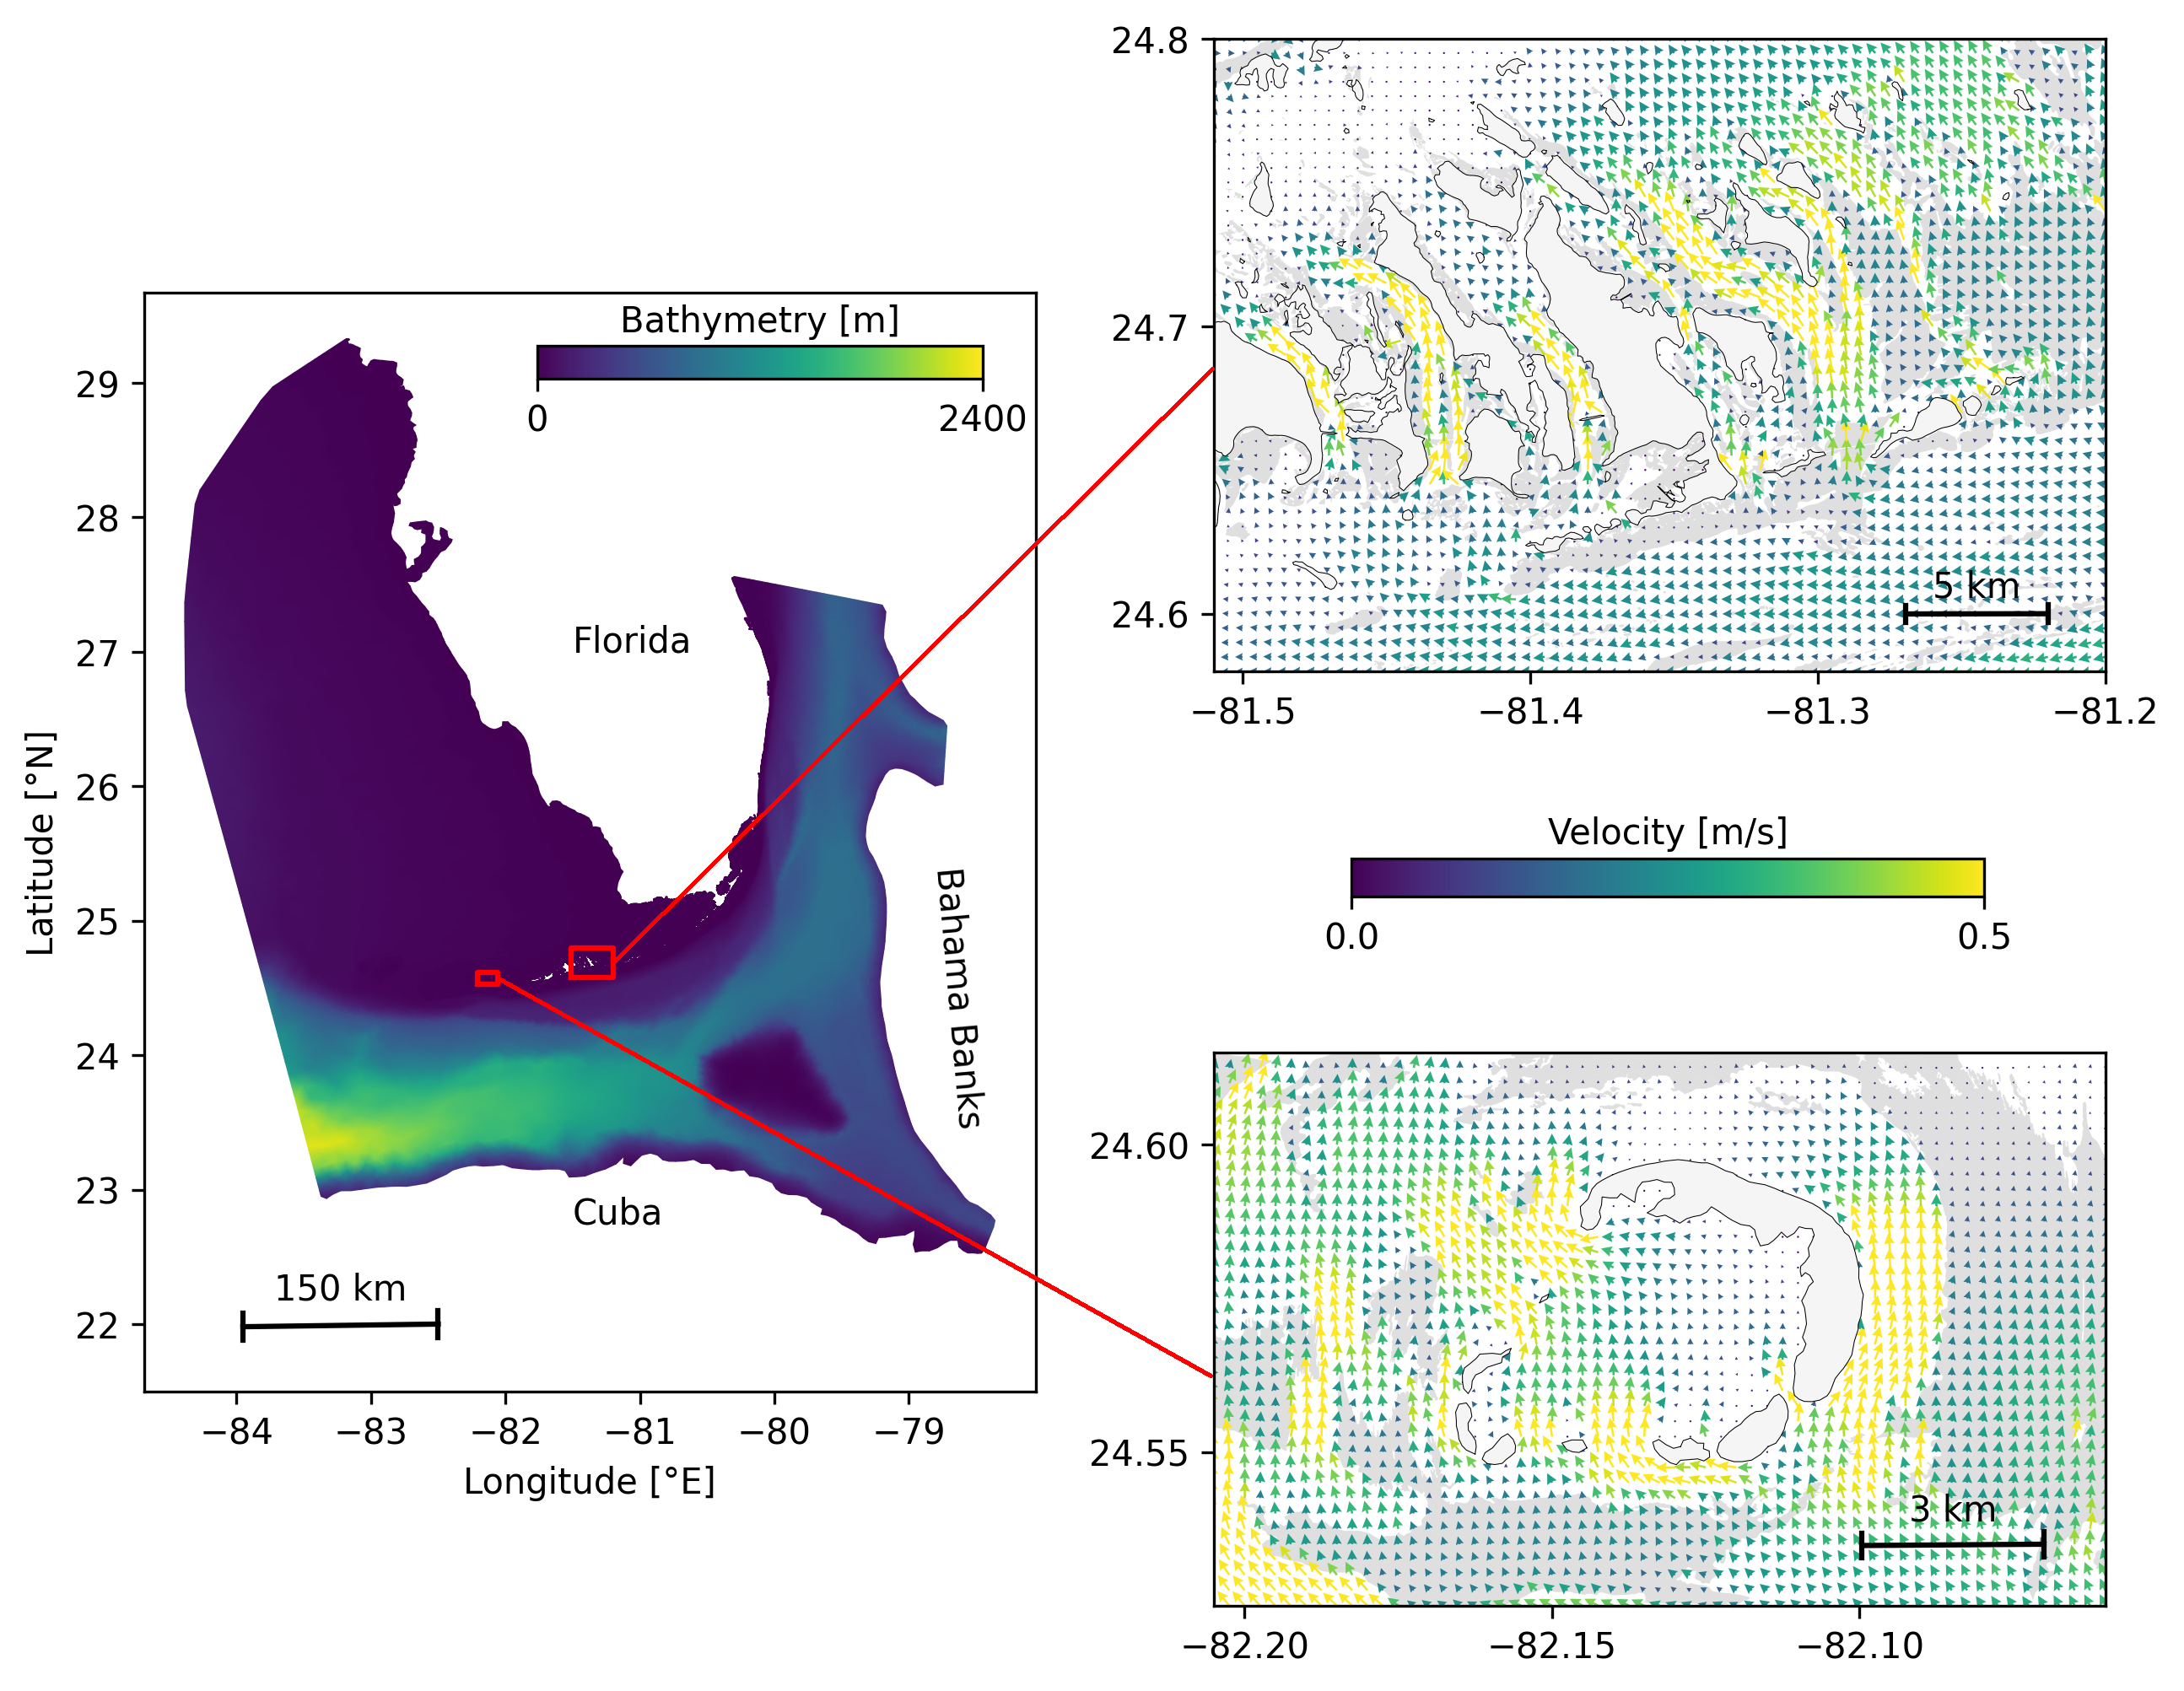
\includegraphics[width=.9\textwidth]{figures/setup_3.png}
    \caption{Model computational domain with the bathymetry (left) and close-up views of the mesh with snapshots of the currents on May, 25 2018 at 00:00, for the Marquesas Keys (bottom) and the Lower Keys (top). This illustrates the benefits of unstructured meshes to represent the fine-scale details of the topography and hence simulate currents down to the scale of individual reefs (shown in light grey) and islands (shown in black).}
    \label{fig:setup}
\end{figure}

The mesh resolution depends only on the distance to the coast but we distinguish between the coastlines along the FRT where we impose a maximum resolution of 100 m and the other coastlines along which the maximum resolution is 2500 m. The mesh has been generated with the open-source mesh generator GMSH \citep{Geuzaine2009} and has about $7 \times 10^5$ elements. The coarsest elements, far away from the FRT, have a size of about 10 km. An illustration of ocean currents simulated on that mesh are shown in Fig. \ref{fig:setup}. It shows how a 100-m spatial resolution allows us to simulate fine-scale details of the flow, such as recirculation eddies and currents within the dense reef system in the Lower Keys that consist of many individual reefs with narrow passages in between. 

The simulated currents can then be used to model dispersal of infectious material throughout the FRT. In this study, 3 types of potential vector carrying the disease causative agent were considered: positively buoyant (e.g. mucus and surfactant), neutrally buoyant (e.g. fines, pelagic organisms) and negatively buoyant (e.g. sediments, composites, demersal organisms). As SLIM is a depth-averaged model, the mean currents it generates are well suited to model the dispersal of neutrally buoyant material remaining within the water column. However, these currents must be modified to correctly represent the dynamics of materials evolving in the surface and bottom boundary layers. Therefore, surface current response to winds is estimated by adding 1.5\% of the wind speed to SLIM currents with a windage angle of 45$^\circ$ to the right for positively buoyant particles. Such parametrization is shown to be an accurate approximation of wave-induced Stokes drift and quasi-Eulerian surface currents by \citep{ardhuin2009observation}. For negatively buoyant materials, on the other hand, bottom currents are obtained by taking 60\% of SLIM currents velocity with a veering angle of 15$^\circ$ to the left \emphc{(explain why)}\textcolor{blue}{TD: Ekman ? Check with Lew...}.

Using these three velocity fields, virtual particles are then released on all the reefs composing the FRT to model the dispersal of infected materials carrying the disease causative agent. The locations of the reefs of Florida are extracted from the "coral reefs and hardbottom" layer of the Unified Florida Reef Tract Map \citep{fwc2017unified}. The polygon of this reef map are then further divided into 500 m squares in order to track the propagation of the disease with a finer geographical resolution, generating a total of 16823 polygons. % \textcolor{red}{(14058 without the big Vaca reef)}
At the beginning of each simulated months and for each type of currents, a total of about $1.5 \times 10^6$ particles are released over all the reef polygons. These particles have a state composed of their polygon of origin as well as their mass, initialized to 1, that they loose at a constant rate $\gamma$ as they are moved by surface, mean or bottom currents. \textcolor{blue}{As monthly simulations are performed, the value of $\gamma$ is chosen so that particles have a half life of 30 days}. When the particles are brought over reef polygons by currents, the amount of infected mass that lands on the polygon is recorded in monthly potential connectivity matrices whose entries are denoted $C_{ij}$. The matrix rows correspond to the source reefs and the columns correspond to the destination reefs. Hence $C_{ij}$ represents the mass of infected material originating from sub-reef i that has settled on sub-reef j. This matrix is then normalized by dividing each of its rows $i$ by the the total mass of particles released on polygon $i$ in order to obtained the normalized potential connectivity matrix $\tilde{C}$, whose entry $\tilde{C}_{ij}$ gives the probability that infectious material produced on sub-reef $i$ settles on sub-reef $j$. Connectivity matrices are computed for each type of current and for each month of the simulated period.

% --> Subsection 2
\subsection{Epidemiological modeling}
% --> Subsubsection 2.1
\subsubsection{Model equations}
The spread of the SCTLD throughout the FRT is simulated using a connectivity-based Kermack-McKendrick SIR model \citep{brauer2008compartmental}. SIR models are among the most standard epidemiological models. They divide individuals into three compartments: susceptible (S), infectious (I) and removed (R). When affected by the disease, susceptible individuals become infectious and infect other susceptible individuals until they are removed, either by recovery or death. Such models usually rely on the hypothesis of an homogeneous, well-mixed population. To account for the spatial heterogeneity of the FRT, the basic SIR formulation is here modified by considering the proportions of susceptible ($S_j$), infectious ($I_j$) and removed ($R_j$) corals of each polygon reef $j$. In this epidemiological model, individual reefs interact through the exchange of infectious material as represented by the connectivity matrix. For each sub-reef $j$ and at any time, the following relations hold: $0\leq S_j,I_j,R_j\leq 1$ and $S_j+I_j+R_j=1$. The evolution of these proportions through time is governed by the following equations:
\begin{equation}
    \begin{aligned}
% * <thomas.dobbelaere@uclouvain.be> 18:19:36 18 May 2020 UTC+0200:
% Birth/death rate ???
        \dfrac{dS_j}{dt} &= -\beta\sum_i\dfrac{A_i}{A_j}I_i\tilde{C}_{ij}S_j - \beta'(I_j)S_jI_j \\
        \dfrac{dI_j}{dt} &= \beta\sum_i\dfrac{A_i}{A_j}I_i\tilde{C}_{ij}S_j + \beta'(I_j)S_jI_j - \sigma I_j \\
        \dfrac{dR_j}{dt} &= \sigma I_j
    \end{aligned}\label{eq:epidemio}
\end{equation}
where $\tilde{C}_{ij}$ is the entry of reef $(i,j)$ of the normalized potential connectivity matrix [-], $A_i$ is the area of reef polygon $i$ [km$^2$], $\sigma$ is the removal rate [day$^{-1}$], and $\beta$ and $\beta'(I_j)$ are the inter- and intra-reef disease transmission rates [day$^{-1}$], respectively. In this model, infectious corals of reef $i$ can infect corals of reef $j$ if there is non-zero probability of infectious material exchange from reef $i$ to reef $j$, given by $\tilde{C}_{ij}$. Moreover, to account for coral resistance to the disease, the intra-reef transmission function $\beta'(I_j)$ has the shape of a smooth step function of the proportion of infectious corals $I_j$ and writes:
\begin{equation}
    \beta'(I_j) = \dfrac{\beta_0'}{2}(1+\tanh[(I_j-I_0)/\tau]),\label{eq:beta}
\end{equation}
where $I_0$ is a threshold on the infection population above which intra-reef transmission becomes significant, and $\tau$ is a measure of the interval over which the transition for low to high transmission occurs. As long as the proportion of infectious corals on reef $j$ is below $I_0$, the only infection mechanism taking place is connectivity-driven transmission at rate $\beta$. Once the threshold is exceeded ( $I_j \geq I_0$ ), intra-reef transmission with rate $\beta'_0$ is activated. A larger value of threshold $I_0$ corresponds to a greater resistance to disease for corals and therefore a slower spread of the disease within reef $j$. Coral birth and natural (\ie non SCTLD-related) death rates are not take into account in this model, as they are assumed to balance each other. This assumption seems reasonable since coral populations of the FRT were declining prior to the emergence of the SCTLD outbreak. For this study the same values were used for $\beta$ and $\beta'_0$.

\subsubsection{Calibration}
Transmission and removal parameters of $\sigma$ and $\beta_0'$ are fitted to observations in order to accurately simulate the temporal evolution of $S_j,I_j,R_j$ on each infected reef polygon. \textcolor{blue}{[some details about parameter estimations from the meta-analysis would be nice here]}

To relate our model framework to the compiled data, Eqs $\ref{eq:epidemio}$ are simplified to a single-reef SIR system:
\begin{equation}
    \begin{aligned}
        \dfrac{dS}{dt} &= -\beta'_0SI \\
        \dfrac{dI}{dt} &= \beta'_0SI - \sigma I \\
        \dfrac{dR}{dt} &= \sigma I
    \end{aligned}\label{eq:simplified}
\end{equation}
Due to the low values of the entries of the normalized connectivity matrix $\tilde{C}_{ij}$, intra-reef transmission, when activated, is the dominant infection mechanism of Eq. \ref{eq:epidemio}. Consequently, Eqs. \ref{eq:simplified} give a reasonable approximation of the evolution of the disease on sub-reefs for which $I_j > I_0$. Using this approximation, the ratio $\beta_0'/\sigma$ is imposed by matching the modeled proportion of susceptible corals remaining after the disease has vanished ($S_\infty$) with observations. A standard property of a SIR model solution is that
\begin{equation}
    S_\infty - \frac{\sigma}{\beta_0'}\log(S_{\infty}/S_0) = 1\label{eq:ratio}
\end{equation}
where the initial proportion of susceptible corals is taken equal to $1-I_0$ (see for instance \cite{Murray07}). The obtained $\beta'_0/\sigma$ ratio is then used to find the value of $\beta'_0$ that reproduces the observed temporal evolution of the state of the coral colonies.

\subsubsection{Initialization}
In order to solve Eqs. \ref{eq:epidemio}, initial conditions are needed, \ie proportions of susceptible, infectious and recovered corals at the beginning of the simulated period. This information is constructed based on different field-collected datasets: : (i) Coral Reef Evaluation and Monitoring Project (CREMP; 2014–2017), (ii) CREMP Presence/Absence Data (CREMP P\_A; 2016–2017), (iii) Southeast Florida Coral Reef Evaluation and Monitoring Project (SECREMP; 2014– 2017), (iv) Florida Reef Resilience Program Disturbance Response Monitoring (FRRP; 2014–2017), (v) Hurricane Irma Rapid Reef Assessment (IRMA; 2017, \cite{viehman2018}), (vi) the Southeast Florida Action Network citizen science program (SEAFAN; 2014–2017), and (vii) the Southern Coral Disease Margin field effort (2017; \cite{neely2018surveying}). These datasets give the locations and dates at which the SCTLD has been observed throughout the FRT. Using this information, we first delineate an infected zone by constructing the concave hull of the points where the disease was observed before May 2018. The reefs infected prior to the beginning of our simulated period are then defined as the reefs located inside the constructed zone. The time of observed infection is then spatially interpolated on each reef of the infected zone by kriging with a Gaussian semivariogram using Python \texttt{pyKrige} module. Assuming an initial state $(S,I,R)=(1-I_0, I_0, 0)$ when the disease was observed, the proportions of susceptible, infectious and removed corals on each reef of the infected zone on the 1st May 2018 is finally approximated using the simplified equations \ref{eq:simplified}. Reefs outside of the infected zone are initialized with a population of 100\% of susceptible corals.  
\subsubsection{Computation of front displacement rate}
\begin{figure}
    \centering
    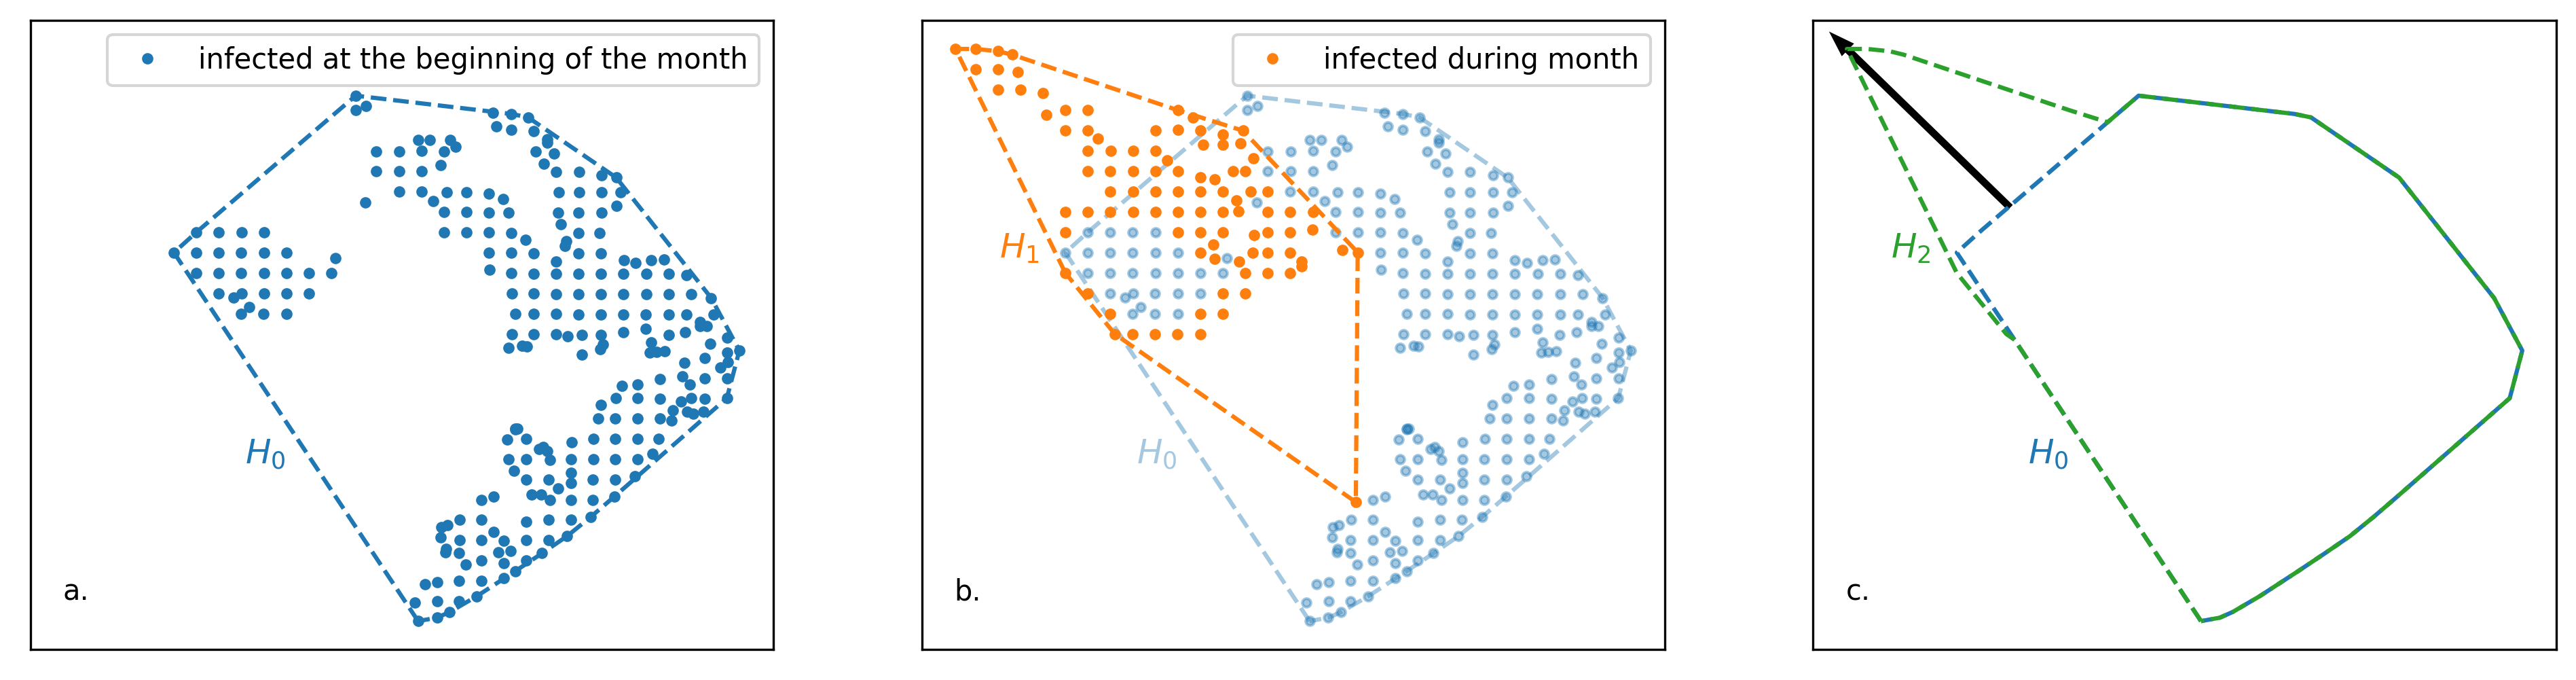
\includegraphics[width=.95\textwidth]{figures/hull_example.png}
    \caption{Method used to compute the disease front displacement during a simulated time interval.\textbf{a.} Concave hull of the infected polygons at the beginning of the simulated period $H_0$. \textbf{b.} Concave hull of the polygons infected during the simulated simulated $H_1$. \textbf{c.} Arrow showing the computed front displacement during simulated time interval between $H_0$ and $H_2$, the union of $H_0$ and $H_1$.}
    \label{fig:hull}
\end{figure}
\citep{muller2020spatial} estimated the speed of the spreading STCLD epidemics at around 92 m/day in the southern section of the FRT. In order to assess our simulation results in regard to this value, we developed a methodology to compute the displacement of the disease front during a given time interval within our simulatzd period. First, the concave hull of the infected polygons at the beginning of the time interval $H_0$ is computed. Then the concave hull of the polygons infected during the time interval $H_1$ is computed while the concave hull $H_2$ is defined as the union of $H_0$ and $H_1$. This methodology is illustrated in figure \ref{fig:hull}. The distance traveled by the disease front is then obtained by computing:
\begin{equation}
    \max\limits_{\mathbf{x}_2\in H_2}\min\limits_{\mathbf{x}_0\in H_0} \|\mathbf{x}_2 - \mathbf{x}_0\|_2
\end{equation}
The epidemics front speed is finally computed by dividing the resulting distance by the number of days in the simulated time interval.

% === RESULTS === %
\section{Results}

\subsection{Exchanges of infected materials}
Connectivity matrices are obtained for mean, bottom and surface currents for all simulated months. These matrices can be more easily handled by interpreting them as large graphs whose vertices are reefs. Such networks can then be analyzed using graph theory tools such as the weighted connectivity length (WCL), \ie the average dispersal distance from origin to destination for material produced on a given reef. The weighted connectivity of reef polygon $j$ writes:
\begin{equation}
    WCL_j = \dfrac{\sum_i \tilde{C}_{ji} L_{ji}}{\sum_i \tilde{C}_{ji}}
\end{equation}
where $L_{ji}$ is the distance between reef polygons $j$ and $i$. Another relevant connectivity measure is the local retention, \ie the proportion of elements released on a given reef that settles on the same reef. In addition to these two metric, indicators such as the probability of exchange between reefs as well as the number of outgoing connections per reef can be computed. The mean values of these indicators for each type of currents are given in table \ref{tab:connect}. Bottom currents give the networks with smallest WCL and outdegree, suggesting that they drive infected materials on shorter geographical ranges and fewer reefs that the other two types of currents. This behavior is consistent with bottom currents showing the largest local retention. However, as bottom currents also exhibit the largest average connection probability, they tend to exchange more infectious matter between connected reefs. Mean and surface currents, on the other hand, generate networks with similar WCL. However, although both currents show analogous spreading ranges, exchanges are almost twice smaller with surface currents and occur between less reefs. Furthermore, surface currents exhibit very weak local retention compared to the two other types of current. This is imputable to the effect of the winds that prevent infectious materials to durably settle on reefs.

\begin{table}
    \centering
    \begin{tabular}{|l|c|c|c|}
        \hline
                                   & mean currents      & bottom currents    & surface currents   \\
        \hline
        \makecell{mean weighted \\
        connectivity length [km]}  & 20.63              & 12.25              & 21.39              \\
        \hline
        \makecell{mean exchange 
        \\probability}             & $2.9\cdot 10^{-4}$ & $7.5\cdot 10^{-4}$ & $1.8\cdot 10^{-4}$ \\
        \hline
        \makecell{mean outgoing \\
        degree}                    & 416                & 159                & 321 \\
        \hline
        \makecell{mean local  \\
        retention}                 & 0.001              & 0.0021             & 0.0003 \\
        \hline
    \end{tabular}
    \caption{Mean values of the graph theory indicators used to analyze the connectivity matrices obtained with mean, bottom and surface currents}
    \label{tab:connect}
\end{table}

\subsection{Epidemiological model results}

Best fit to observations is obtained with transmission rate $\beta_0'=6.45$ days$^{-1}$ and removal rate $\sigma=6.99$ days$^{-1}$. Comparison of the evolution of the state described by Eqs \ref{eq:simplified} results with observations is shown in figure \ref{fig:calibration}. Transmission and removal rates are found to have fairly close values with ratio $\beta_0'/\sigma$ being equal to $1.0345$. This proximity in rate values is imposed by Eq. \ref{eq:ratio}, as observations show a proportion of susceptible individuals of about $85\%$ at the end of the outbreak. Since infection and removal occur at very close rates, the instantaneous proportion of infectious individuals on the reefs remains pretty low through the outbreak, with a maximum value of about $0.4\%$.
\textcolor{blue}{[I might come up with some more ideas when figures merged, as it will ease comparisons]}
%These results are in accordance with the characteristic infection time of $\sim 10.5$ days deduced from transmission experiments.

\begin{figure}
    \centering
    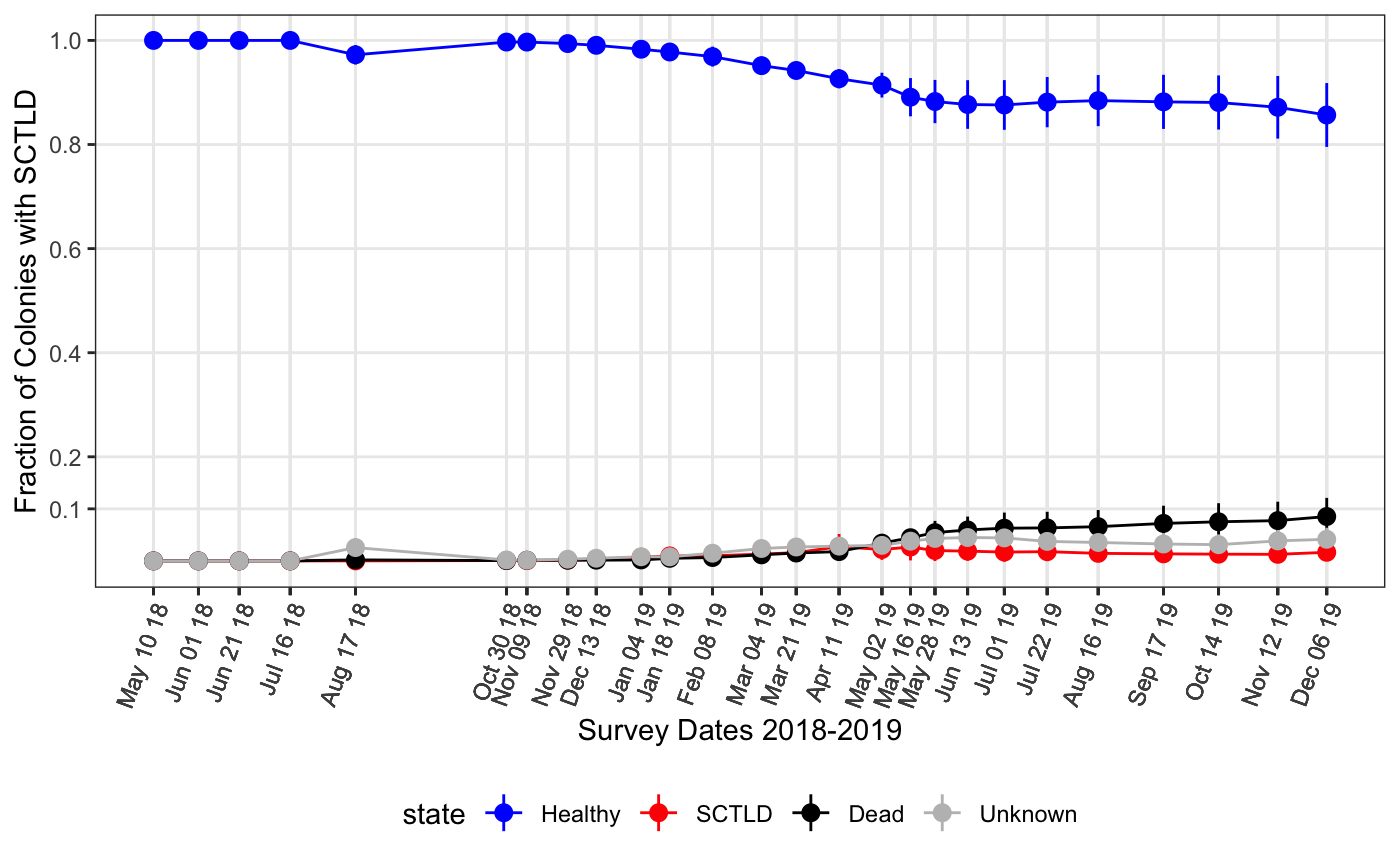
\includegraphics[width=.7\textwidth]{figures/image2.png}
    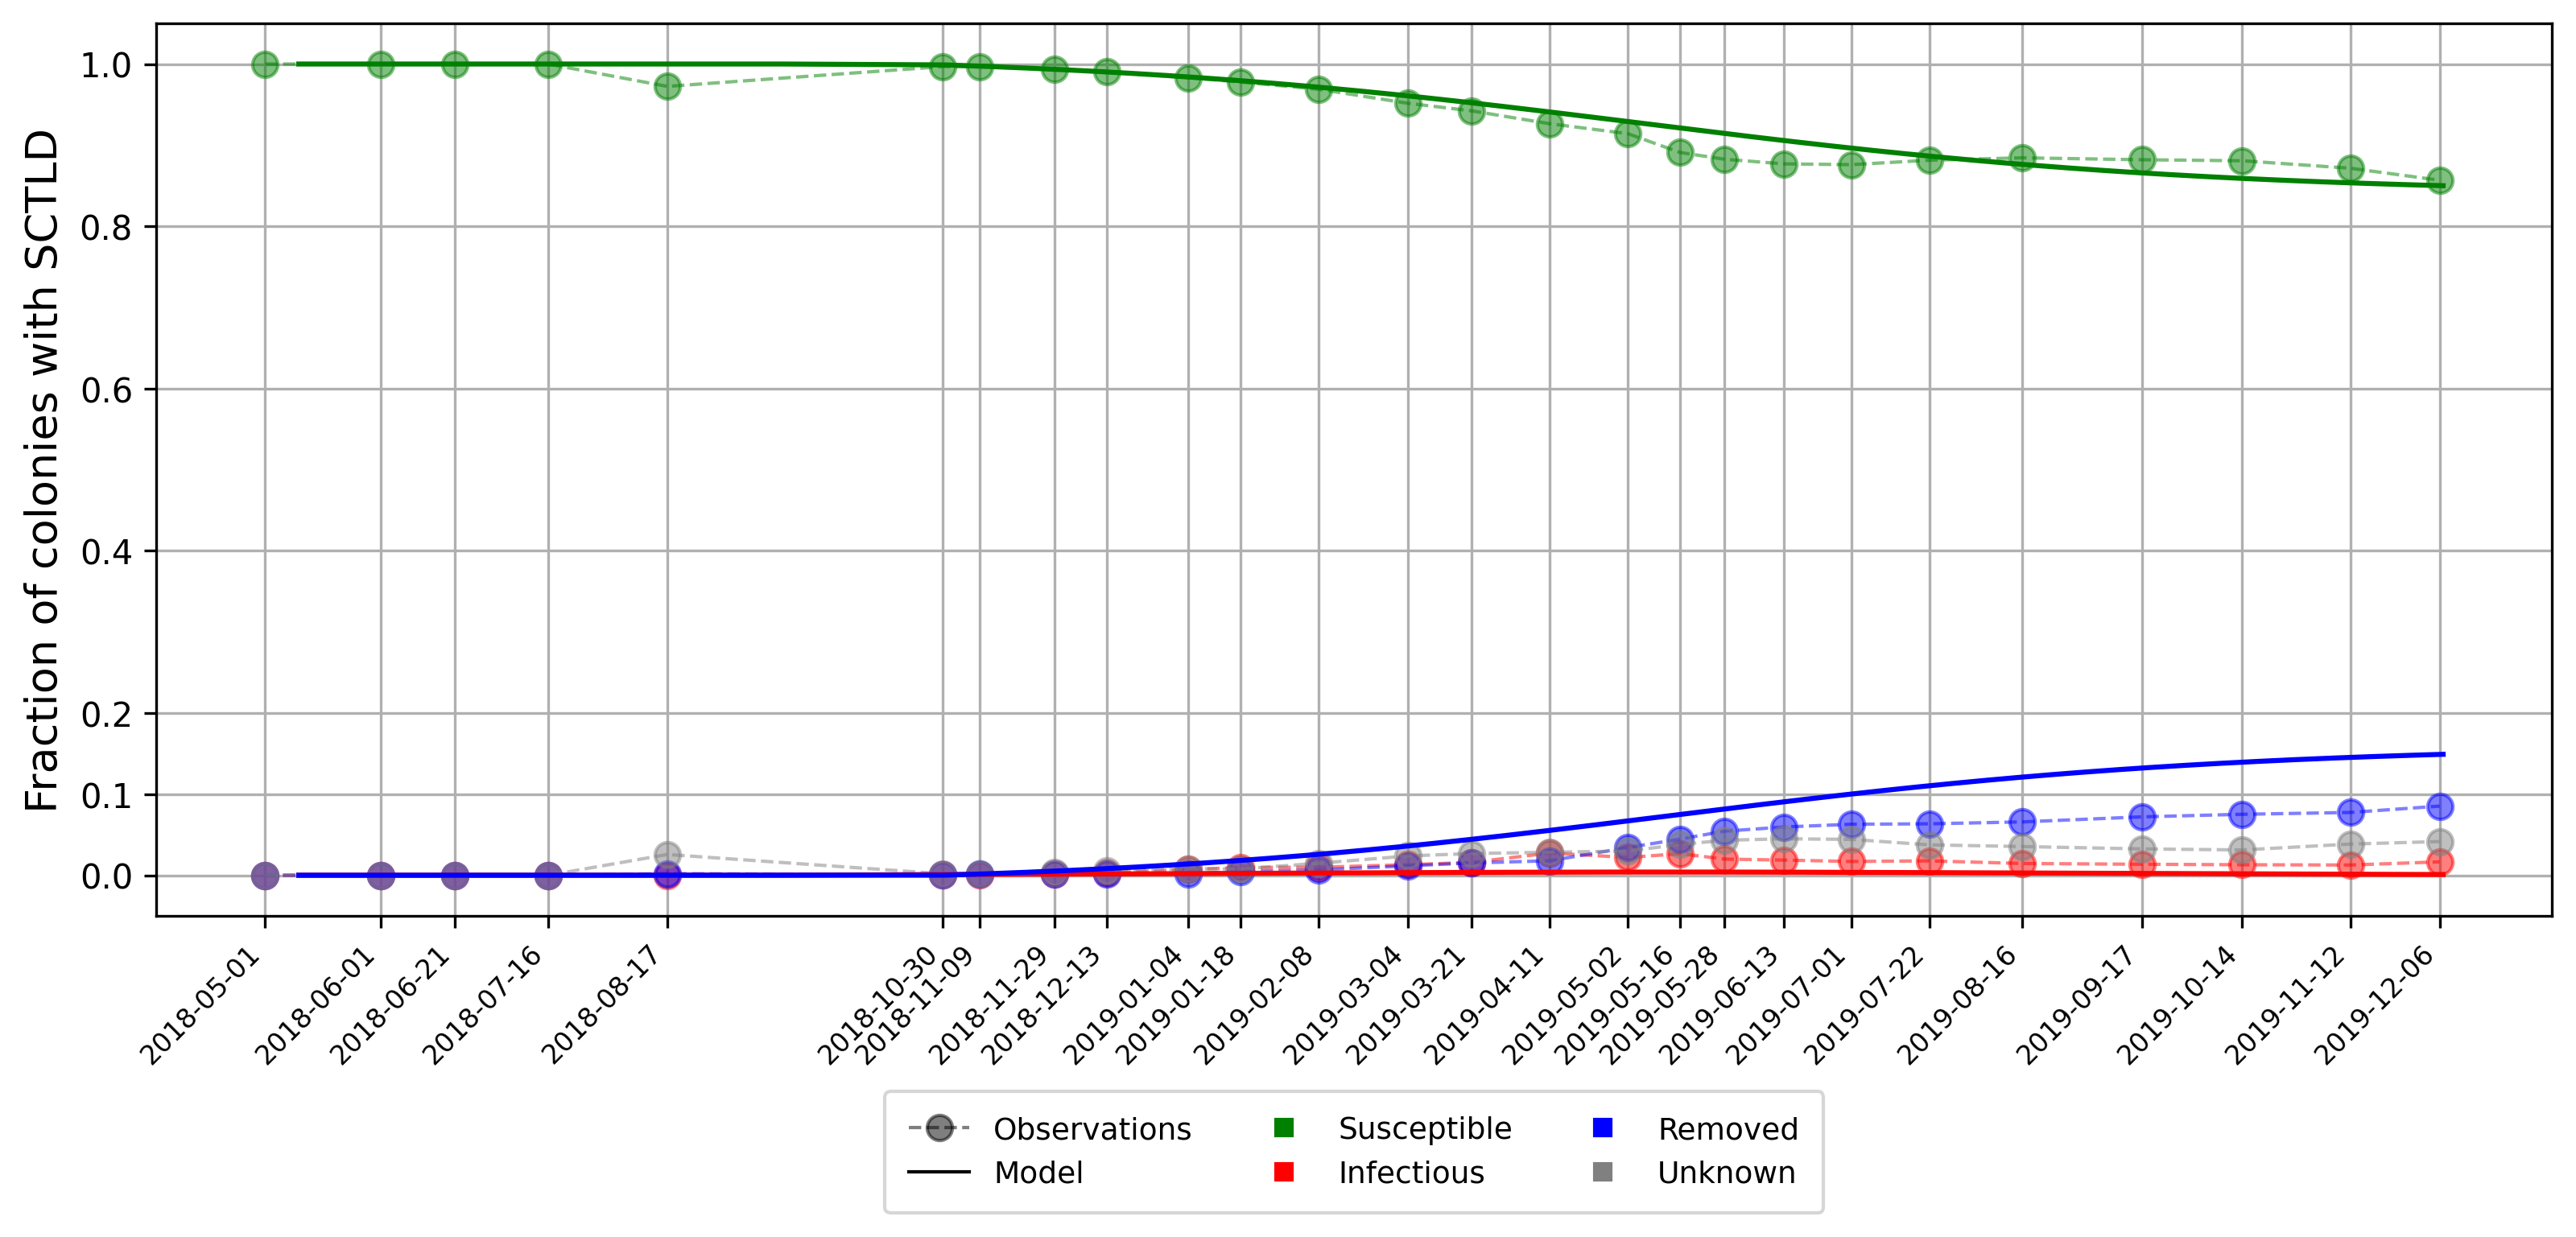
\includegraphics[width=.69\textwidth]{figures/sir_obs.png}
    \caption{\textbf{Above:} Observed disease prevalence over time (all colonies from all sites), error bars are the 95\% confidence intervals. \textbf{Below:} Disease prevalence over time as modeled by Eqs. \ref{eq:simplified} using calibrated transmission and removal parameters  $\beta_0'=6.45$ days$^{-1}$ and $\sigma=7$ days$^{-1}$.}
    \label{fig:calibration}
\end{figure}

Using the above calibrated epidemiological parameters, epidemiological model simulations were performed for each type of currents and different values of the infection threshold $I_0$. A summary of the simulation results are shown in figure \ref{fig:results}. Two metrics are used to assess the accuracy of the model. First, the modeled front speed is compared to the reference rate of 92 m/day derived by \citep{muller2020spatial}. Furthermore, we compute the mean of the distances between each point where the SCTLD has been observed during our simulated period and the centroid of the closest reef polygon predicted to be infected by our model during the same period. Figure \ref{fig:results} show that mean barotropic currents outperform other types of current regarding both criteria with a front speed of 107 m/day and a mean accuracy of $\slim ~1.2$ km; while surface currents produce the worst results with respect to both front speed and proximity to the observed affected reefs.

Moreover, results of Fig. \ref{fig:results} show a strong dependence to infection threshold $I_0$. Front speeds of both mean and bottom currents reach a plateau for values of infection threshold between $I_0=0.05\%$ and $I_0=0.1\%$, while the minimal prediction error is attained around $I_0 \approx 0.078\%$ with mean currents. For $I_0 > 0.1\%$, intra-reef infection is strongly impeded and populations of infectious individuals on infected reefs are not sufficiently large to infect other colonies on reefs they are connected to. For values of $I_0$ lower than $0.05\%$ on the other hand, intra-reef infection dominates and coral population on infected reefs is removed too fast to efficiently spread the disease through the network. Model results suggest that propagation of the disease only occurs for fairly small values of $\I_0$, implying low coral resistance to the causative agent of the SCTLD. 

\begin{figure}
    \centering
    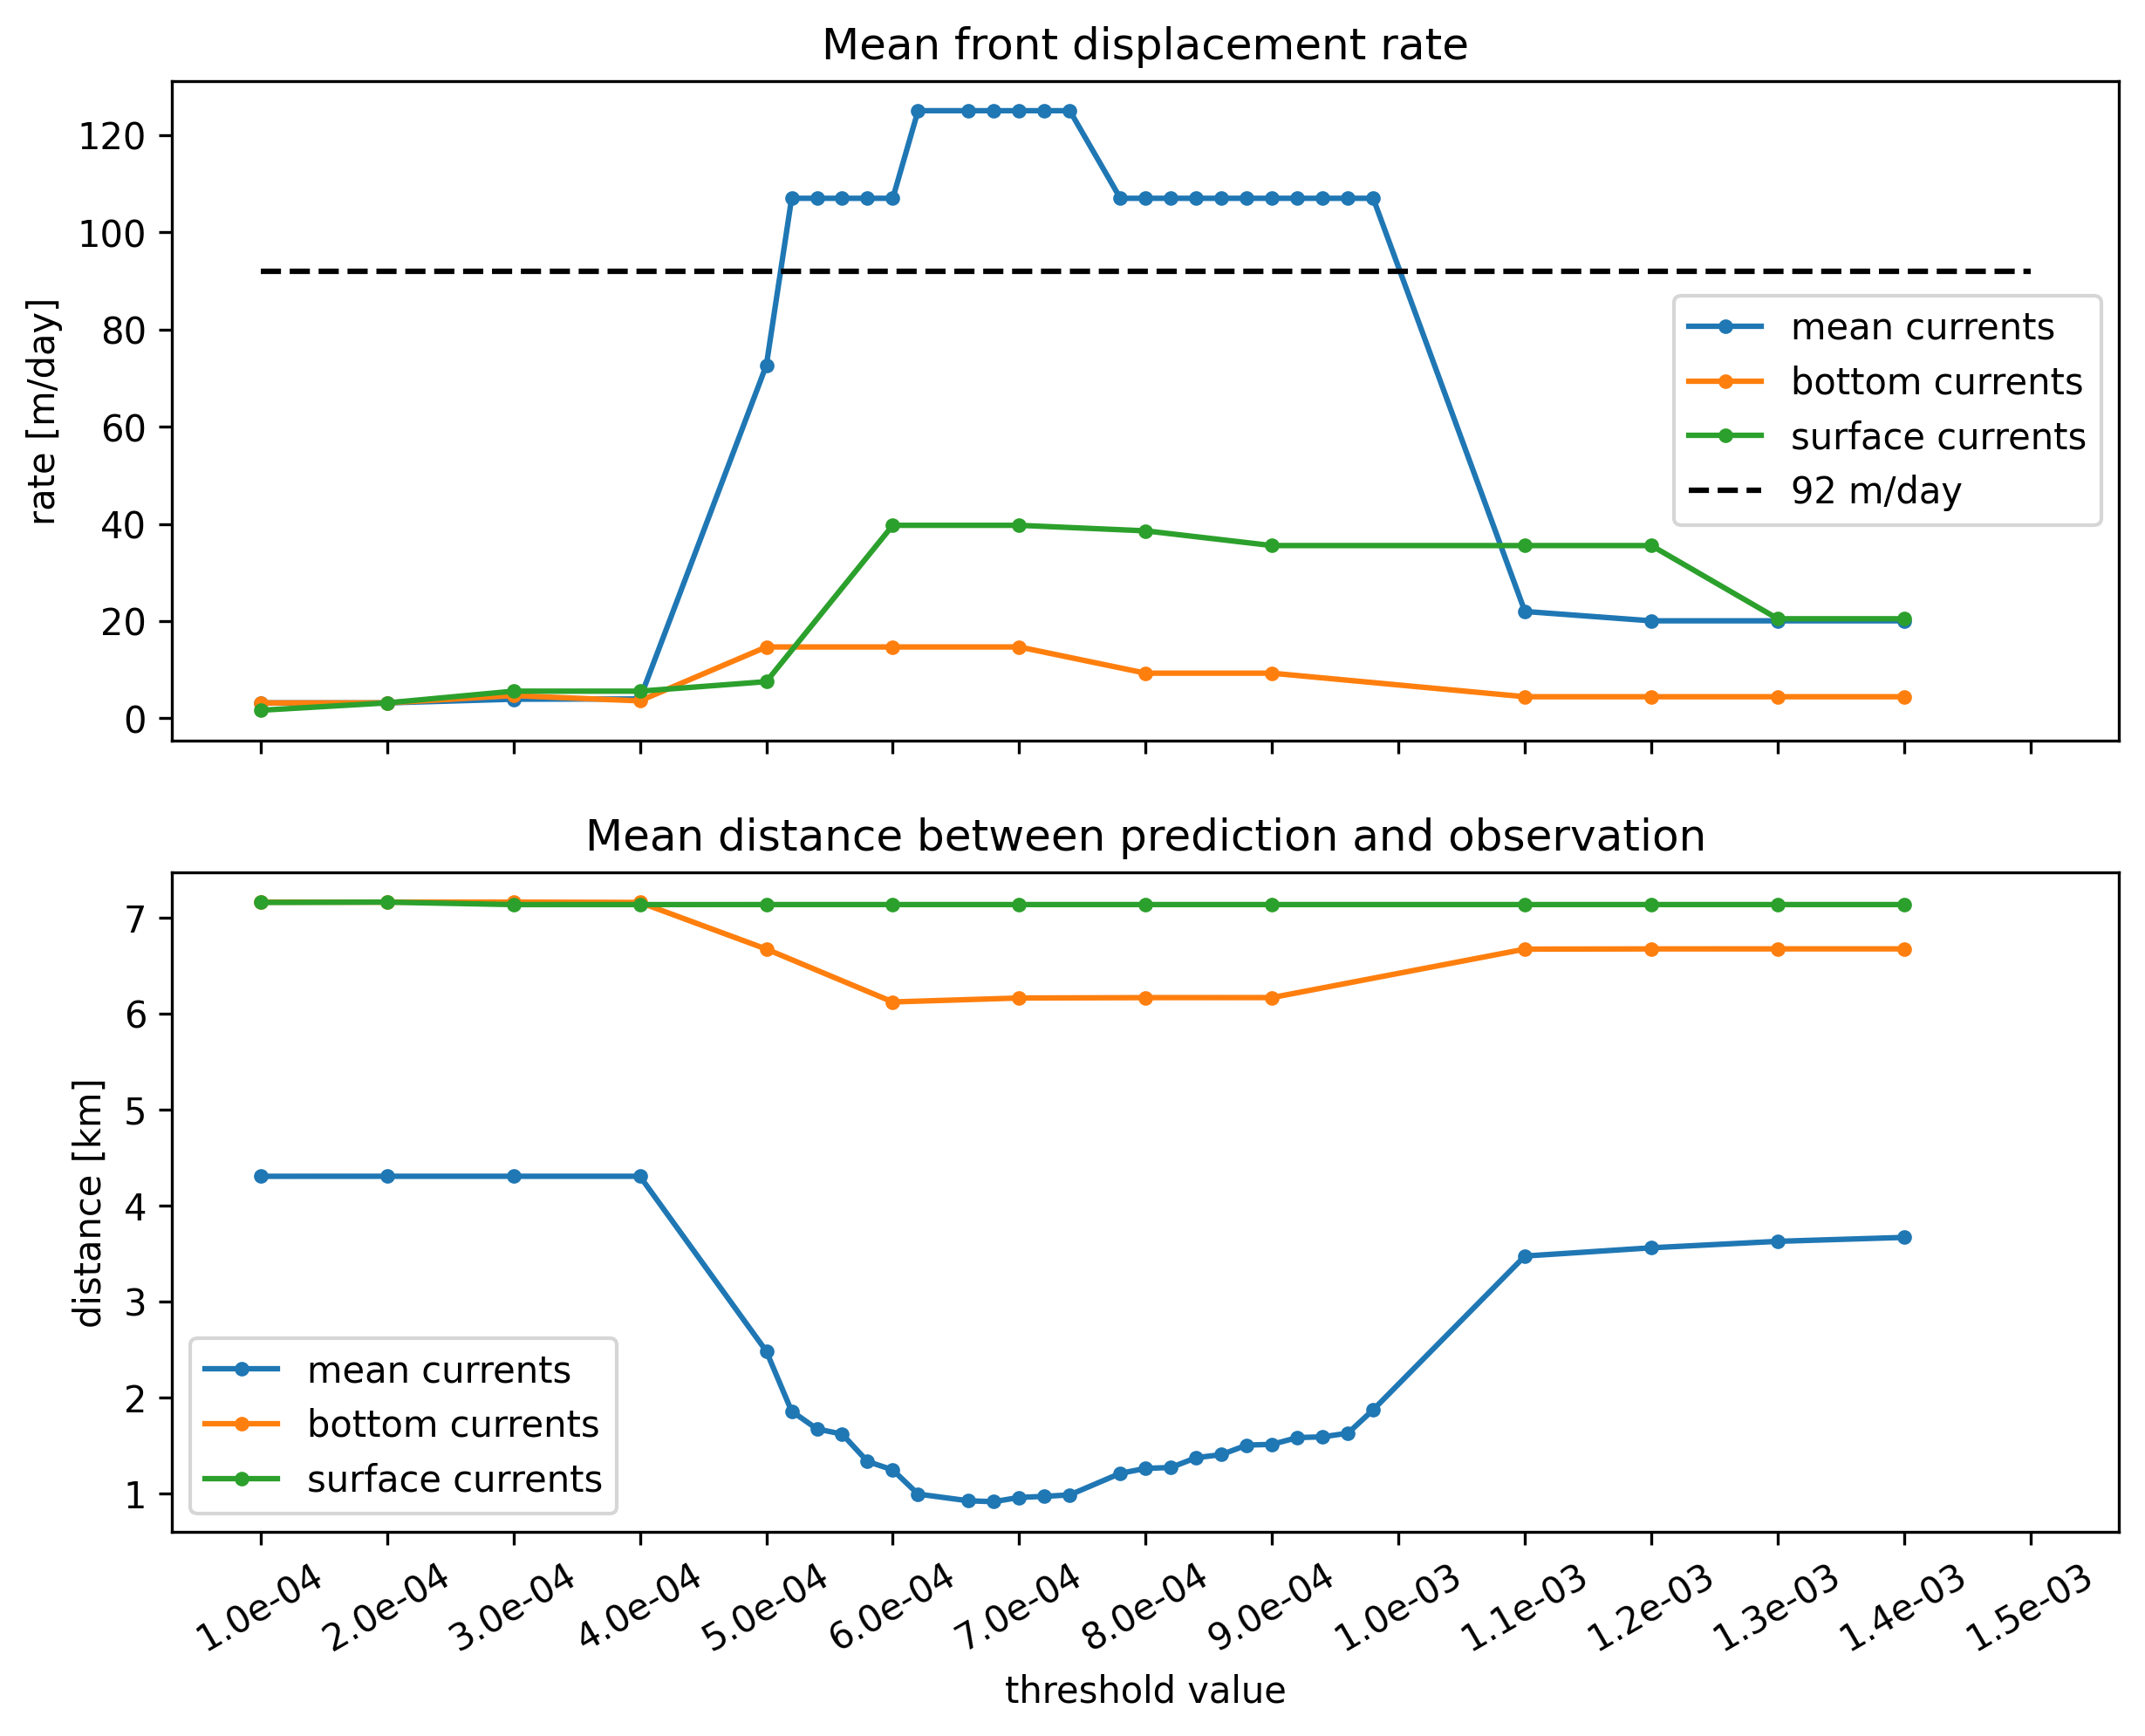
\includegraphics[width=.8\textwidth]{figures/sctld_validation_corrected.png}
    \caption{Summary of epidemiological model simulations with calibrated transmission parameters. \textbf{Top:} Modeled disease front speed for each type of current with respect to intra-reef infection threshold $I_0$. \textbf{Bottom:} Mean distance between predicted infected reefs and observed disease points. These results show that mean barotropic currents outperform other modes of transport at reproducing the observed spread of the disease. The appearance of a plateau suggests that model predictions are very sensitive to the value $I_0$}
    \label{fig:results}
\end{figure}

The differences between the three modeled types of currents shown in figure \ref{fig:results} can be explained by analyzing the trajectories of the particles used to model the transport of the vector of the causative agent of the disease, as illustrated in Fig. \ref{fig:traj}. Due to the impact of wind on positively buoyant materials, particles driven by surface currents are likely to be blown away from the reefs (see upper part of Fig. \ref{fig:traj}). Moreover, even when winds are pushing particles along the reef line, these particles spend less time over the same region than particles driven by mean and bottom currents (see lower part of Fig. \ref{fig:traj}. Smaller amounts of particle mass will therefore settle on reef polygons, leading to lower entries of the potential connectivity matrix, \ie lower exchange probabilities between reefs. Hence, despite being able to displace infected materials on greater distances, surface currents are less likely to drive the propagation of the disease. Particles driven by bottom currents, on the other hand, remain longer over the same region, producing larger entries of the potential connectivity matrix. Due to these large exchange probabilities between reefs, bottom currents are better at propagating the disease (Fig. \ref{fig:results}). Nevertheless, bottom currents being relatively slower, exchanges of infected materials occur on a limited geographical range. Mean barotropic currents, that carry particles on greater distances while allowing for sufficiently large amounts of infected mass to settle on reef polygons, are thus best suited to propagate the disease (Fig. \ref{fig:results}).

The results shown in figure \ref{fig:results} were obtained by removing the large reef located North to Vaca key, denoted Vaca reef as in \cite{frys20}, from our reef polygons. Preliminary simulations showed that this reef has close to no impact on the modeled spread of the disease to the rest of the FRT, as it sends few infectious matters to southerly and easterly neighboring reefs. Moreover, Vaca reef has a low coral coverage ($0-10\%$), which strongly impedes disease spread on the reef. However, as coral coverage is not taken into account in our epidemiological model, propagation of the disease on the reef was overestimated. This led to unrealistically strong modeled front speed variations due to the large size of the reef. Consequently, and in the absence of SCTLD observations on Vaca reef, it has been removed from our reef polygons in order to avoid overestimation of the disease spread.

\begin{figure}
    \centering
    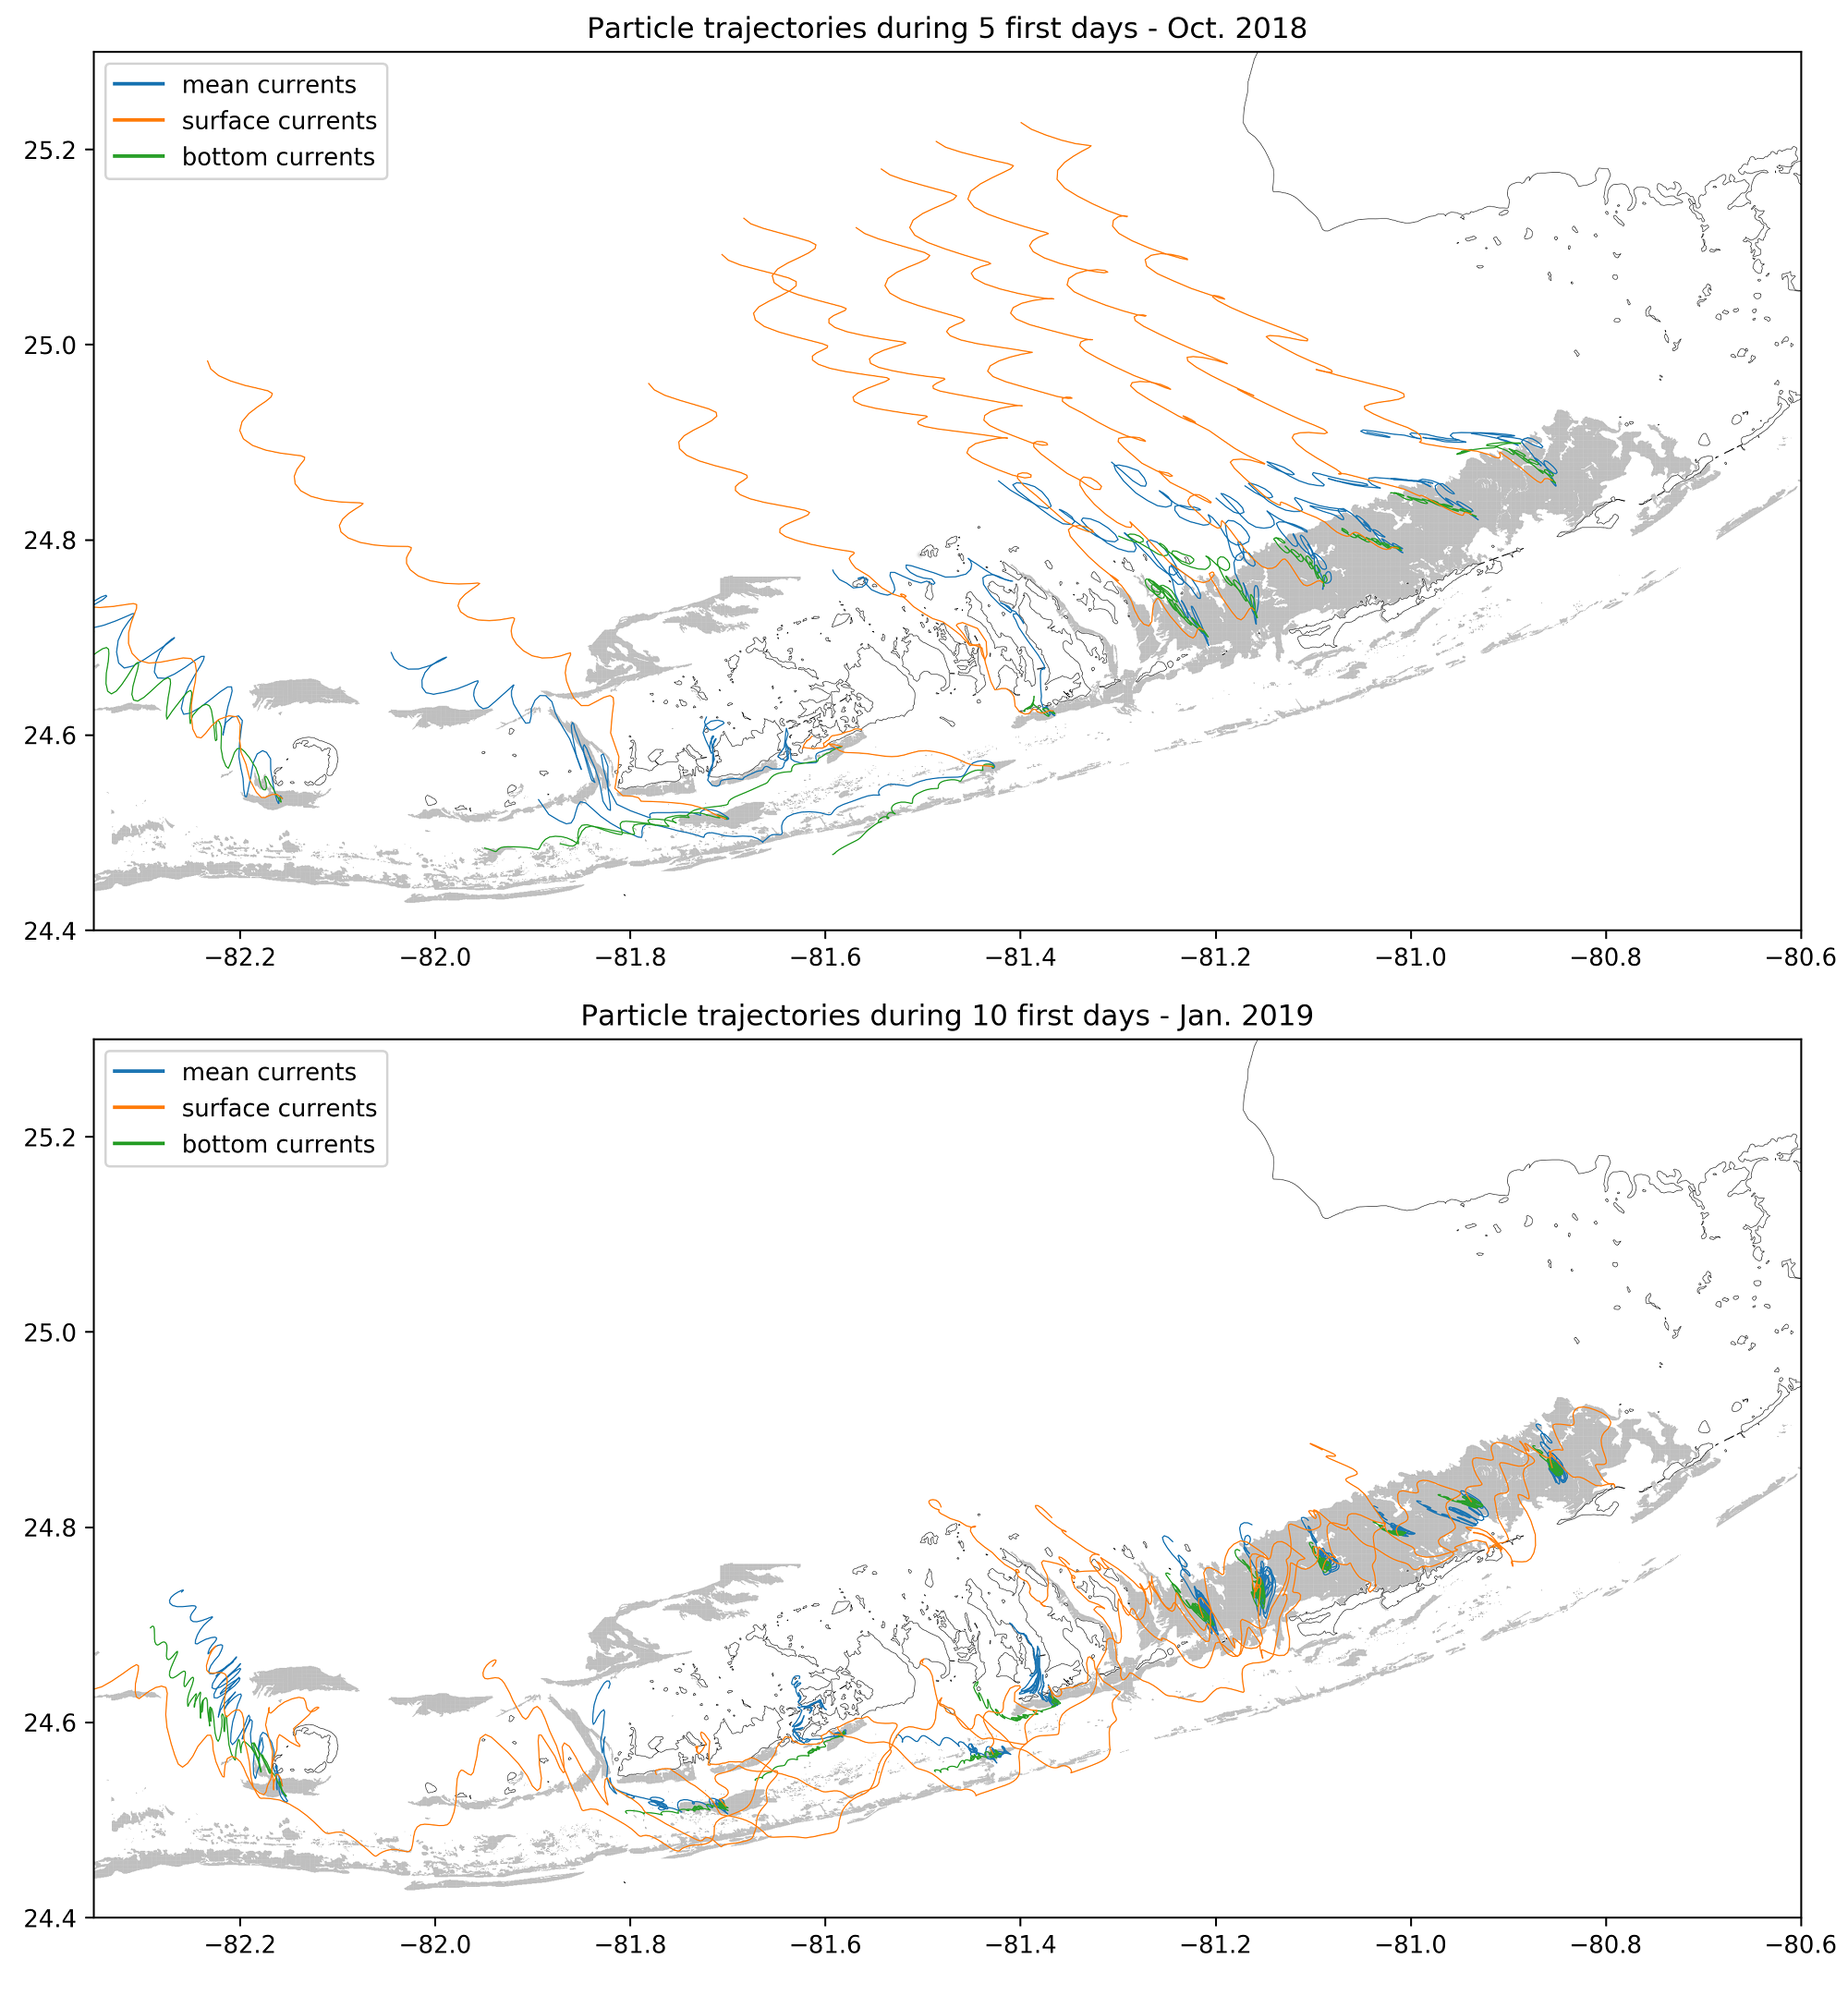
\includegraphics[width=.9\textwidth]{figures/traj.png}
    \caption{}
    \label{fig:traj}
\end{figure}

%\begin{figure}[h]
%    \centering
%    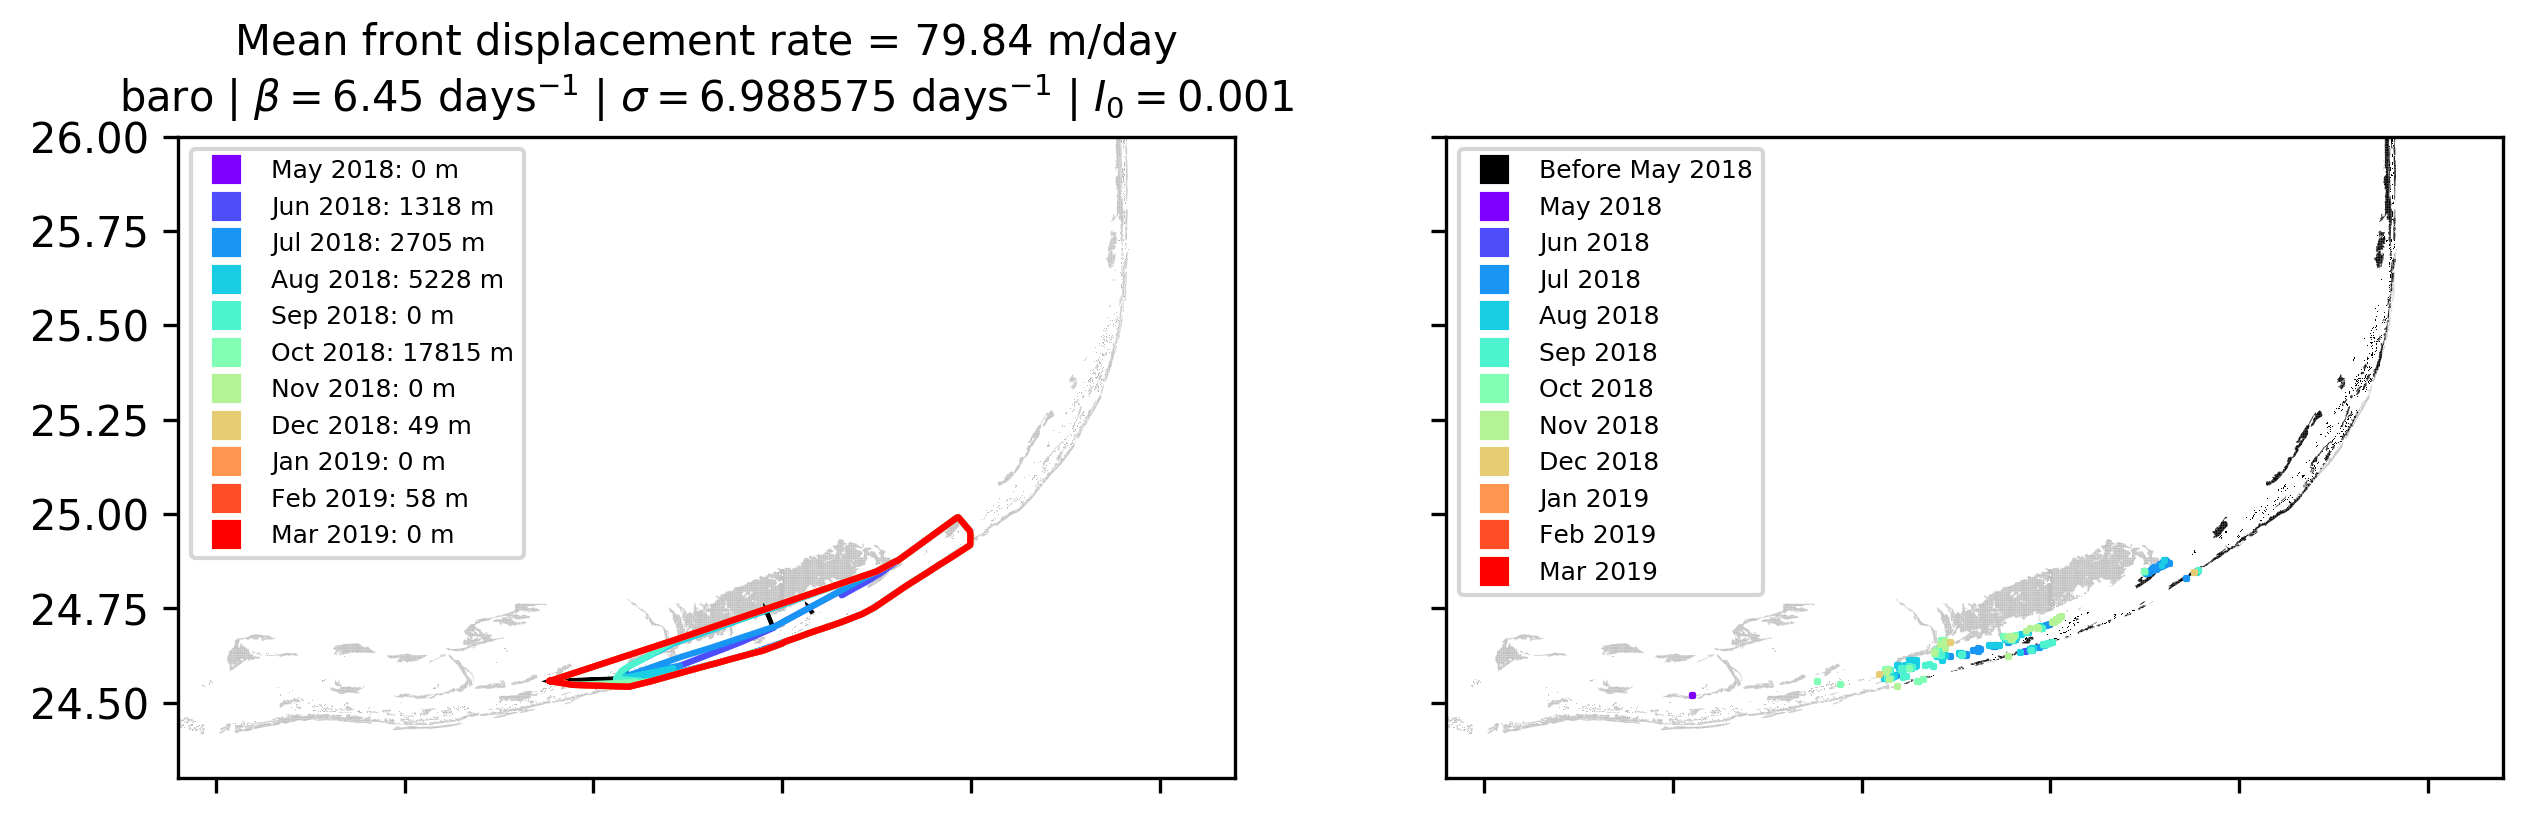
\includegraphics[width=.9\textwidth]{figures/hull_result.png}
%    \caption{Take home messages:\begin{itemize}
%        \item Our methods accurately captures disease front evolution through time (mtch between points and concave hulls)
%    \end{itemize}}
%    \label{fig:front}
%\end{figure}

% === DISCUSSION === %
\section{Discussion and conclusions}

%% --- SUMMARY OF TAKE HOME MESSAGES --- %%

Calibrating our model with observations, we found a characteristic transmission time of 6.45 days as well as a removal rate of 6.99 days for the SCTLD. Feeding this parameters to the model, our simulation suggest that only mean current are able to reproduce the observed spread o the disease. Bottom current do not spread infectious matter on a sufficient geographical range while surface currents do not allow infected elements to settle durably on reefs. This therefore suggests that the causative agent of the SCTLD disease might be transported within neutrally buoyant materials inside the water column. Assuming this mode of transport, propagation of the disease from reef to reef only occurs for a narrow range of values of infection threshold $I_0$. This threshold is defined as the maximum proportion of infectious corals that a colony can withstand without the disease to spread. As disease spread occurs for threshold values of in the range $0.05-0.1\%$, this suggests that corals have low resistance to the SCTLD.

%% --- DISCUSSION OF TAKE HOME MESSAGES/MAIN RESULTS --- %%

% 1. MODEL PARAMETERS
After calibration with observations, the value of the ratio $\beta_0'/\sigma$ between intra-reef and removal rates is given by $1.0835$. This value being close to 1, modeled infectious individuals are removed from the system almost as fast as susceptible individuals get infected. This causes the proportion of infectious corals on the reefs to remain pretty low (\ie $\leq 0.4\%$) through time. This suggest that only a small fraction of the colony causes the disease to spread on the reef during the outbreak. \textcolor{blue}{[add some comments on tank experiments and say that they give transmission time within same order of magnitude]}. In this study, the same values were used for inter- and intra-reef rates $\beta$ and $\beta_0'$. This implies that the infectiousness of the causative agent is not reduced during its journey from reef to reef. However, to assess the impact of this assumption, epidemiological model simulations were performed with $\beta=\beta_0'/2$. The resulting disease front speeds did not exceed 20 m/day. This strong decrease can be explained by the interplay between inter- and intra- reef infection. Reducing inter-reef transmission rates decreases the proportion of infectious corals on reefs attained by infectious materials, which in turn reduces the amount of infectious matter sent to the rest of the network. This suggests that, to reproduce the observed spread, inter- and intra-reef transmission rates must have similar magnitude, \ie that the causative agent is barely not degraded while travelling from reef to reef.

% 2. MEAN BAROTROPIC CURRENTS => NEUTRALLY BUOYANT VECTOR 
Model suggests causative agent transported by neutrally buoyant materials
\begin{itemize}
    \item What would be candidates for vector then ?
    \item Is there another known disease with similar spread mechanism ?
    \item Talk about ballast waters study (bottom currents) (?)
    \item potential disagreement with \citep{rosales2020rhodobacterales} for which sediments might be a source of transmission  
\end{itemize}

% 3. IMPACT OF I0/APPEARANCE OF PLATEAU
Coral resistance to the SCTLD in represented by parameter $I_0$, defined as the maximum proportion of the colony that can get infected without causing the disease to spread to the rest of the colony. The modeled propagation of the disease is highly sensitive to this parameter. On the one hand, when corals are strongly susceptible to the disease, infectious individuals are removed from the system too fast to become sustainable sources of infectious materials in the network. On the other hand, if corals are weakly susceptible to the disease, very few corals get infected and the disease barely propagates. Our simulations suggest that this value must be fairly low (around 0.01\%) in order for the disease to spread from reef to reef. \textcolor{orange}{This seems to imply that susceptible coral species have very weak defense mechanisms against the causative agent of the disease. (?)} \\
\textcolor{blue}{TO DO: link $I_0$ to pathogenic load}

%% --- SENSITIVITY ANALYSIS --- %%


% impact of gamma parameter (=limited impact)
%In this model, the half life of the causative agent and its vector is proportional to the inverse of particle mass deposition rate $\gamma$, ans is assumed to be 30 days. In the absence of data on $\gamma$, this assumption seems reasonable as particles life span would match the duration of the monthly simulations used to derive potential connectivity matrices \textcolor{blue}{(Any reference on degradation rate of organic matter in seawater ?)}. Nonetheless, the impact of $\gamma$ was assessed by performing Lagrangian tracking experiments of particles with a half life of 15 days. Increasing $\gamma$ strengthens short range connections while weakening short range connections. However, the decrease of long range connection probability remains limited as both values of $\gamma$ gave matrices with similar weighted connectivity lengths. Moreover, close to no variation was observed in reefs outdegrees. Therefore, although good calibration of $\gamma$ would give more accurate estimations of the probabilities of exchanges of infected materials over short distances, variation of this parameter should have minor impact on the conclusions of our simulations.
% * <thomas.dobbelaere@uclouvain.be> 18:56:49 18 May 2020 UTC+0200:
% Problem of monthly simulations ?

%% --- LIMITATION AND POTENTIAL IMPROVEMENTS OF THE MODEL --- %% (should be reduced)
% 1. Limitations of hydro
As with any modeling study, it is important to understand the assumptions on which the model is based. Here, we have used a 2D barotropic ocean model coupled with the 3D model HYCOM \citep{Chassignet2007} in order to indirectly represent baroclinic phenomena. Such model is well suited to simulate the fate of neutrally-buoyant matters in shallow regions. However, as depth-averaged currents do not accurately approximate the motion of particles in the bottom and surface layers, \slim velocities have been modified to simulate the exchanges of negatively and positively buoyant matters. Surface current response to wind parametrization is based on the results of \cite{ardhuin2009observation}, consistent with observations. In this study, measured surface currents are shown to be in the order of $1.0\% - 1.8\%$ of the wind speed, in a direction $10^\circ - 40^\circ$ to the right of the wind. \textcolor{red}{[TO DO: bottom currents]}. Although such estimation of surface and bottom currents is disputable, using a 2D model allows for reef-scale resolution throughout the whole FRT. Such high-resolution allows to capture recirculation eddies around islands and reefs, that significantly impact the weighted connectivity length as well as the local retentions on the reefs.

% 2. Limitations of epidemiological model
The appearance of an interval of optimal values of threshold $I_0$ for the propagation of the disease in our results highlights the impact of coral resistance on the spread of SCTLD through the FRT. Therefore, a further step in our modeling approach would be further dividing coral populations of our polygons into highly susceptible (\eg \textit{Dichocoenia stokesii}, \textit{Meandrina meandrites}), intermediately susceptible (\eg \textit{Orbicella faveolata}, \textit{Montastrea cavernosa}), and weakly susceptible (\eg \textit{Acropora Palmata}, \textit{Acropora cervicornis}) sub-populations. The proportions susceptible, infectious and removed individuals within these sub-populations would then be modeled with specific transmission ($\beta$, $\beta_0'$) and removal ($\sigma$) rates as well as specific infection thresholds $I_0$. Such approach would however require a fine knowledge of the distribution of the different coral species throughout the FRT. This knowledge about coral coverage could also be used to avoid overestimation of the front propagation, as in the case of Vaca reef.

%% --- NICE FINAL PARAGRAPH --- %%
\textcolor{blue}{TO DO: Conclusion} \\
Part 1: Questions developed in introduction are answered\\
Part 2: Model results complements field observations and tank experiments, bringing new insight to disease management
\begin{itemize}
    \item As our model results are continuous through time, it can exhibit the variability of the propagation of the SCTLD through time and therefore bring additional insight to observation data.
\end{itemize}
% === APPENDIX === %
%\appendix
\section*{Appendix}

% --- MODEL FORMULATION --- %   
\subsection*{Subsection 1}
% --- MODEL EVALUATION --- %
\subsection*{Subsection 2}

\section*{Conflict of Interest Statement}
The authors declare that the research was conducted in the absence of any commercial or financial relationships that could be construed as a potential conflict of interest.

\section*{Author Contributions}
  
\section*{Funding}
This paper is a result of research funded by the Florida Department of Environmental Protection under award XXX to Mote Marine Laboratory. 

\section*{Acknowledgments}
Computational resources were provided by the Consortium des \'Equipements de Calcul Intensif (\textsc{c\'eci}), funded by the \textsc{f.r.s.-fnrs} under Grant No. 2.5020.11.

\section*{Supplemental Data}

% === BIBLIOGRAPHY === %
\bibliographystyle{frontiersinSCNS_ENG_HUMS} 
\bibliography{./biblio.bib}

%%% Make sure to upload the bib file along with the tex file and PDF
%%% Please see the test.bib file for some examples of references

\section*{Tables and figures}


\end{document}
